\documentclass{fetch-my-doc}
\usepackage{tabu}
%\usepackage{multirow}
\usepackage{siunitx}
%\usepackage{enumitem}
%\usepackage{fancyvrb}
%\usepackage{breakurl}
%\usepackage{tocloft}
%\usepackage{pdflscape}
%\usepackage{ltxtable}
%\usepackage{filecontents}
\usepackage{onimage}

\sisetup{output-decimal-marker = {,}}

\definecolor{darkgreen}{rgb}{0,.5,0}

\hypersetup{breaklinks,colorlinks=true,citecolor=darkgreen,urlcolor=blue,linkcolor=blue,anchorcolor=blue} %,pdftex=true}

\newcommand{\hypref}[1]{\SaveVerb{myverb}|#1|\hyperlink{#1}{\protect\UseVerb{myverb}}}

\newcommand{\sep}{\begin{center}\noindent\rule{.5\textwidth}{0.5pt}\end{center}}

\newcommand{\rc}{\rowcolor{lightgray!40}}
\newcommand{\cc}{\columncolor{lightgray!40}}

\makeatletter
\newcommand*{\shift}[2]{%
  \settowidth{\@tempdima}{#2}%
  \makebox[\@tempdima]{\hspace*{#1}#2}%
}
\makeatother

% Linebreak nach paragraph
\makeatletter
\renewcommand\paragraph{%
   \@startsection{paragraph}{4}{0mm}%
      {-\baselineskip}%
      {.5\baselineskip}%
      {\normalfont\normalsize\bfseries}}
\makeatother

\def\imagetop#1{\raisebox{2.5em}{\vtop{\null\hbox{#1}}}}

%\renewcommand{\datum}{14.10.2012}
\renewcommand{\datum}{\today}
\renewcommand{\abgabe}{14.07.2014}
\renewcommand{\version}{1.0.0}
	%	Versionierung:
	%	x.y.z
	%	- x hoch bei ?
	%	- y hoch bei größeren Änderungen von ganzen Absätzen.
	%	- z hoch bei kleinen Verbesserungen wie Rechtschreibung, Satzbau, usw.
\renewcommand{\typ}{Dokumentation}
\renewcommand{\titel}{Dokumentation}
\renewcommand{\libdir}{./}
\bibliography{referenzen}

\setcounter{tocdepth}{4}
\setcounter{secnumdepth}{3}

\tikzset{
    image label/.style={
        every node/.style={
            fill=white,
            fill opacity=.5,
            text opacity=1,
            text=orange,
            font=\fontfamily{phv}\selectfont\Large\bfseries}
        }
}

\begin{document}
	\sloppy
	\begin{titlepage}
	\begin{center}
		\vspace*{.7cm}		
		\thispagestyle{FirstPage}
		\textsc{\LARGE \fach}\\
		%\vspace*{.2cm}
		%{\huge Fetch my ball}\\[0.4cm]
		
		
\includegraphics[width=0.85\textwidth]{\libdir img/logo1.pdf}\\
		%\textsc{\Large \gruppe}\\[0.5cm]

		% Titel
		\HRule \\[0.4cm]
		{ \huge \bfseries \titel}\\[0.4cm]
		Version \version	\\
		\HRule \\[1.5cm]

		\vfill
		
		% Autoren
		\begin{tabular}{rcl}
			\toprule
			\mgEinsVorname\ \mgEinsNachname		&&	\mgEinsMail	\\
			\mgZweiVorname\ \mgZweiNachname		&&	\mgZweiMail	\\
			\mgDreiVorname\ \mgDreiNachname		&&	\mgDreiMail	\\
			\bottomrule
		\end{tabular}
		
		\vspace{2cm}

		{\large Abgabe: \abgabe}
	\end{center}
	\addtolength{\textheight}{\versch}
\end{titlepage}
	\addtolength{\textheight}{\versch}
	%%%%%%%%%%%%%%%%%%%%%%%%%%%%%%%%%%%%
	% TODOS ENTFERNEN NICHT VERGESSEN! %
	%%%%%%%%%%%%%%%%%%%%%%%%%%%%%%%%%%%%
	\printtodo
	%%%%%%%%%%%%%%%%%%%%%%%%%%%%%%%%%%%%
	\addtocontents{toc}{\protect\sloppy}
	\tableofcontents
	\clearpage
	
	%\section{Versions- und Änderungsgeschichte}\label{sec:versionsaenderung}
		%\begin{tabularx}{\textwidth}{ccX}
			%\toprule
			%Version			&	Datum						&	Änderungen	\\\midrule
			%1.0.0				&	14.07.2014			&	Erste veröffentlichte Version	\\
			%\bottomrule
		%\end{tabularx}	
		%\clearpage
	
	\rowcolors*{0}{}{lightgray!40}
	
	%%%%%%%%%% Hier beginnt das Dokument %%%%%%%%%%
	\section{Einführung}\label{sec:Einfuehrung}
		\autor{...}
    
    \begin{center}
      \begin{minipage}[t]{.49\textwidth}
        \begin{figure}[H]%
          \centering%
          \caption{blbla}%
          \label{}%
          \includegraphics[width=\columnwidth]{img/ball1.jpg}%
        \end{figure}
      \end{minipage}
      \hfill
      \begin{minipage}[t]{.49\textwidth}
        \begin{figure}[H]%
          \centering%
          \caption{blbla}%
          \label{}%
          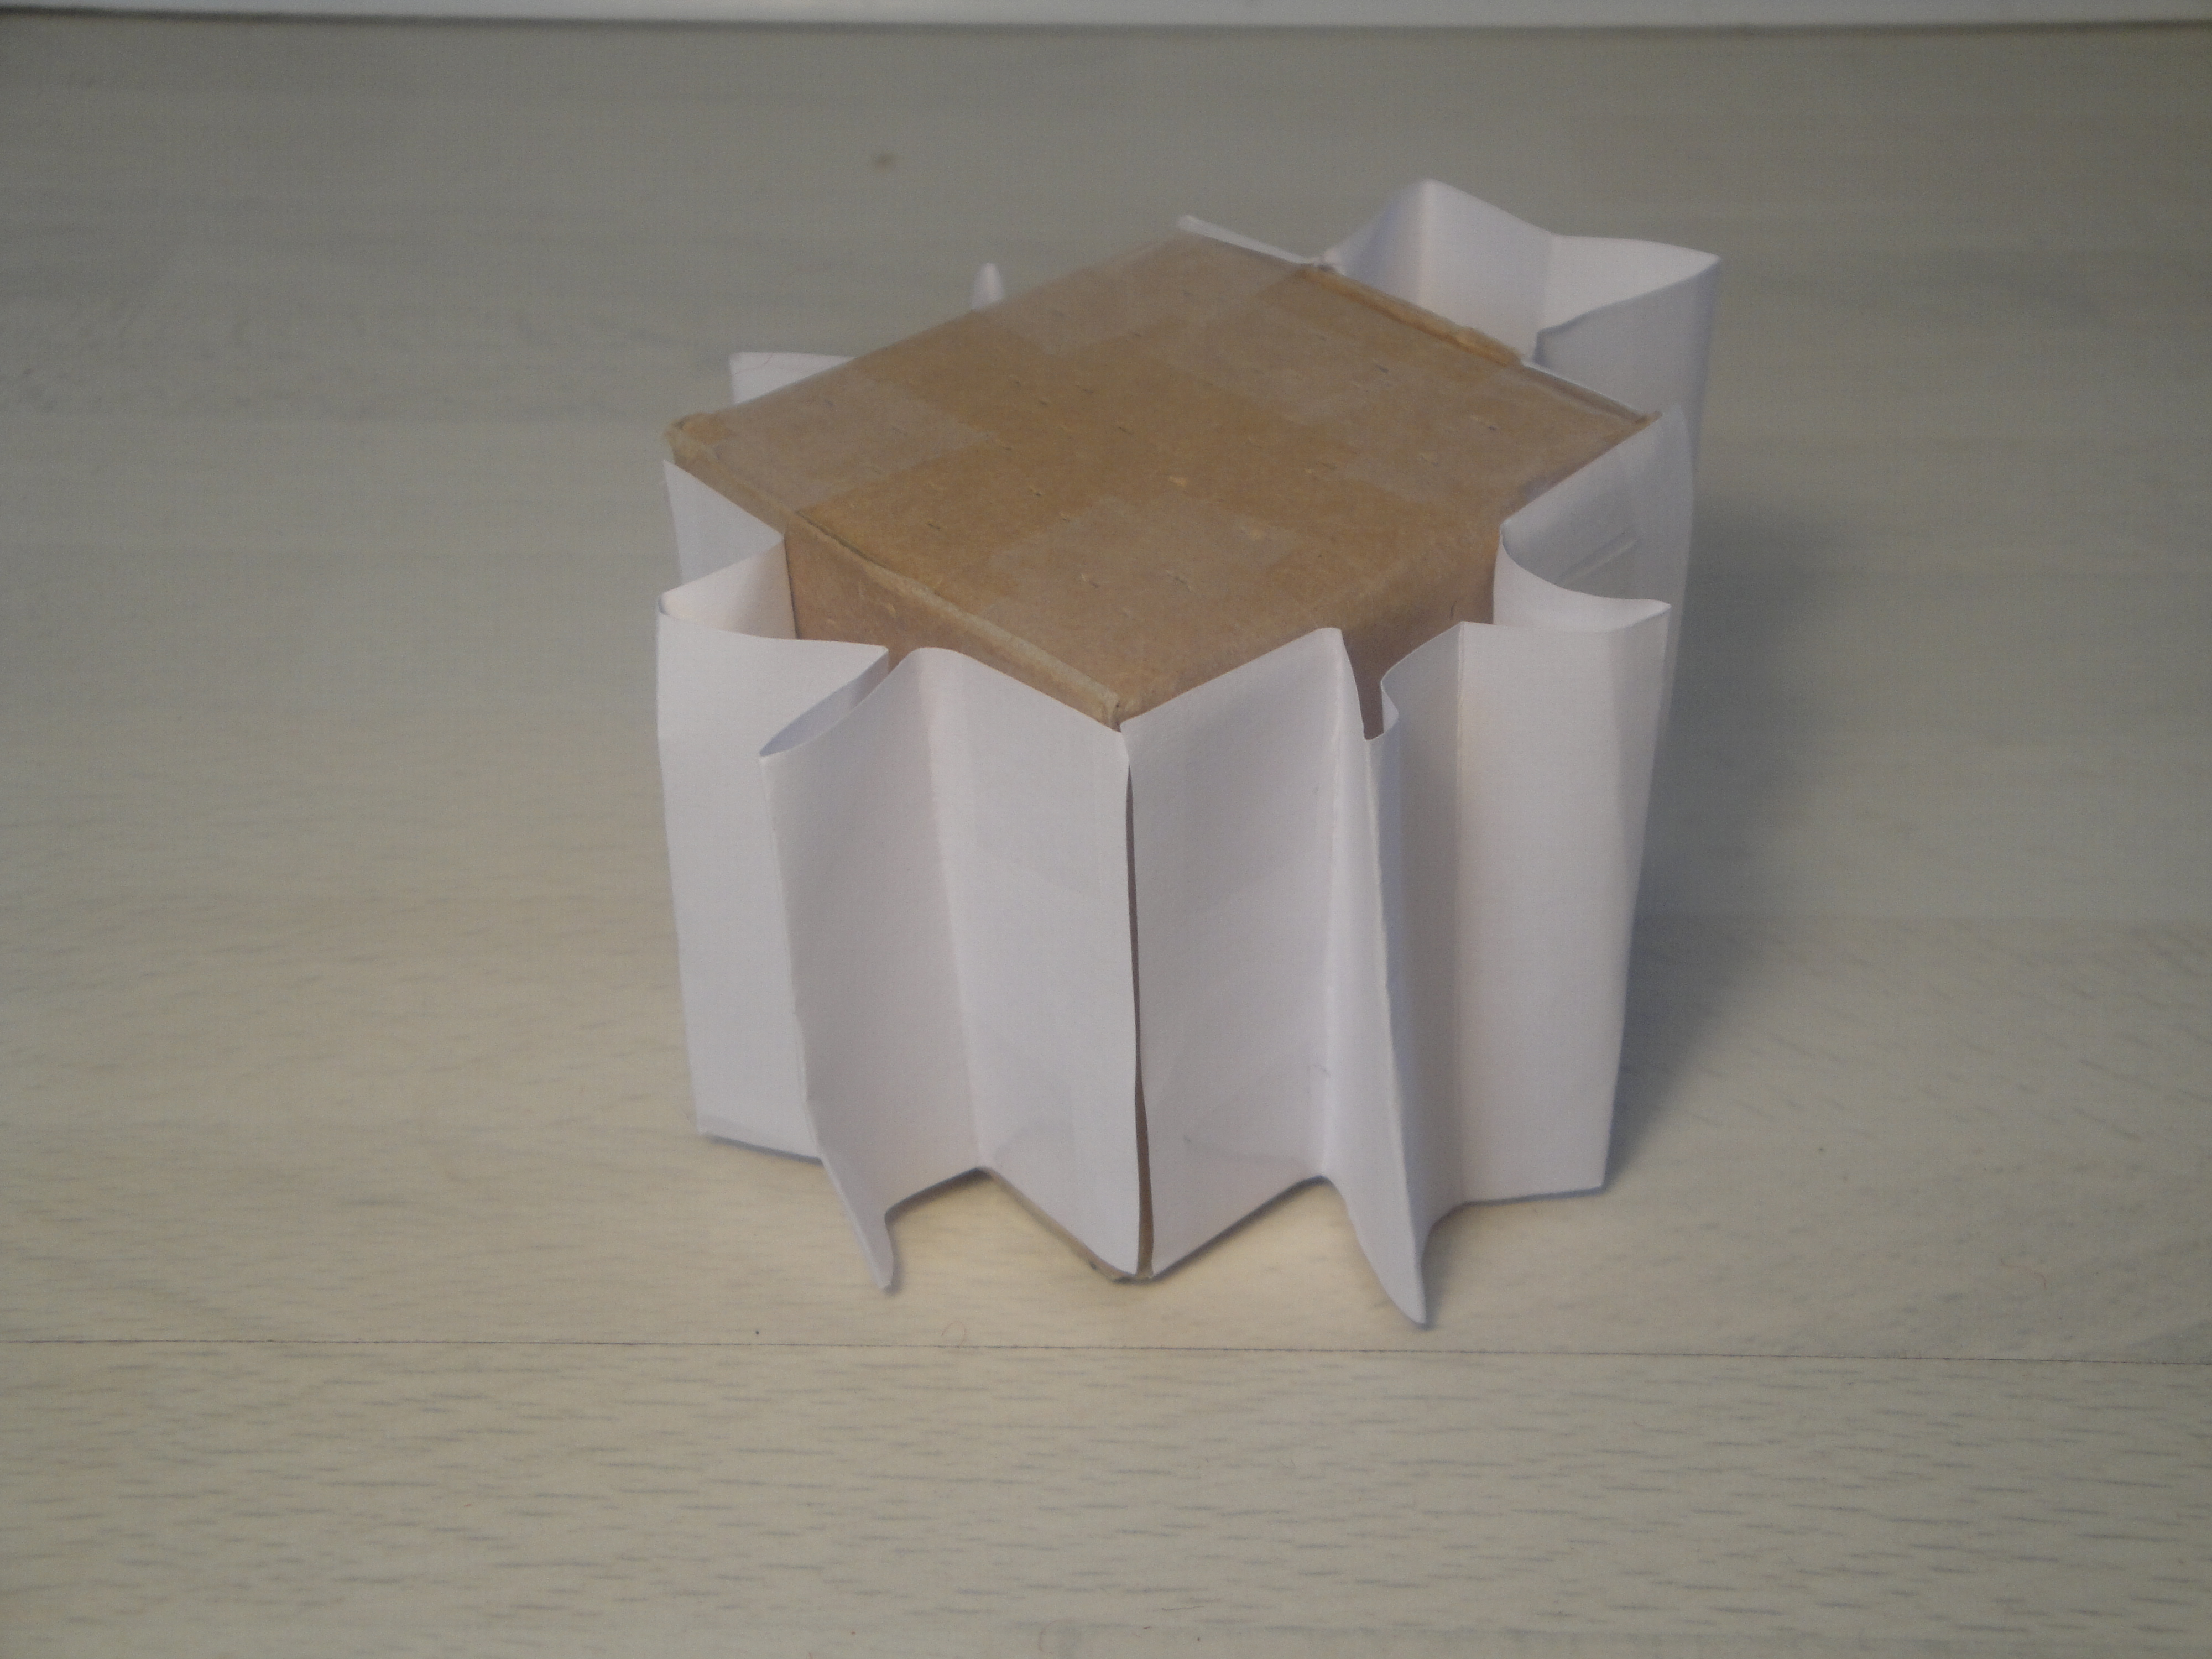
\includegraphics[width=\columnwidth]{img/ball2.jpg}%
        \end{figure}
      \end{minipage}
    \end{center}
    
    \begin{figure}[H]%
      \centering%
      \caption{blbla}%
      \label{}%
      \begin{tikzonimage}[width=\textwidth]{img/robbyOpenSideTop.jpg}[image label]
        \draw [orange, line width=3pt] (0.52,0.37) circle [radius=0.8cm] node [xshift=-1.25cm] {c};
        \draw [orange, line width=3pt] (0.835,0.23) circle [x radius=1.0cm, y radius=1.55cm] node [xshift=-1.5cm] {d};
      \end{tikzonimage}
    \end{figure}
    
    \begin{figure}[H]%
      \centering%
      \caption{blbla}%
      \label{}%
      \begin{tikzonimage}[width=\textwidth]{img/robbyOpenBottom.jpg}[image label]
        \draw [orange, line width=3pt] (0.4,0.39) circle [x radius=2.5cm, y radius=0.85cm] node [xshift=-2.95cm] {a};
        \draw [orange, line width=3pt] (0.4,0.56) circle [x radius=2.5cm, y radius=0.85cm] node [xshift=-2.95cm] {b};
        \draw [orange, line width=3pt] (0.66,0.485) circle [radius=0.8cm] node [xshift=-1.25cm] {c};
      \end{tikzonimage}
    \end{figure}    
    
				
		%\subsection{Referenzen}\label{sec:Referenzen}
			%Es folgt eine Auflistung aller Referenzen zu den im Architekturentwurf erwähnten Fremdressourcen und verwendeten Dokumenten.
				%\printbibliography[heading=none]
		%
		
	%\clearpage
	%\listoffigures
	
	%\listoftables
	%\clearpage
	%\appendix
	
\end{document}